\documentclass[nojss]{jss}
\usepackage[latin1]{inputenc}
\usepackage{longtable}
\usepackage{lscape}
\usepackage{multirow}

\graphicspath{{Figures/}}

\title{Structural Breaks in Inflation Dynamics within the European Monetary Union}

%% for internal use
\newcommand{\fixme}[1]{\emph{\marginpar{FIXME} (#1)}}
\newcommand{\readme}[1]{\emph{\marginpar{README} (#1)}}

% Verkaufsstrategien
% 1. Widerlegung des Teuro Effektes
% 2. Keine Ver�nderung d. EMU sichtbar; nach 2002 kein globaler Trend aller EMU Staaten Richtung Wechsel
% 3. Nutzen zeigen, den die osteurop�ischen Staaten haben, dadurch, dass sie dem EURO beitreten m�ssen  (mit Ausnahme von Slovenien fallender Trend in Mittelwert und Varianz)
% 	 so etwa in Slowenien und der Slovakei ein Bruch bevor diese Staaten dem ERMII/EURO beitreten
% 4. Finanzkrise: schwieriger, ausser Irland keine �nderung > 2008


\author{Thomas Windberger\\Universit\"at Innsbruck \And
        Achim Zeileis\\Universit\"at Innsbruck
}
\Plainauthor{Thomas Windberger, Achim Zeileis}

\Abstract{
  The aim of this paper is to shed some light on the effect of the European Monetary Union (EMU)
  on changing the dynamics of the inflation rates in its Member States. 
}

\Keywords{inflation rate, structural break, EMU}


\Address{
  Thomas Windberger, Achim Zeileis\\
  Department of Statistics\\
  Universit\"at Innsbruck\\
  Universit\"atsstra�e 15\\
  6020 Innsbruck, Austria\\
  E-mail: \email{Thomas.Windberger@student.uibk.ac.at}, \email{Achim.Zeileis@R-project.org} \\
}


\begin{document}


\section{Introduction}

The European Central Bank (ECB) defines price stability ``as a year-on-year increase in the Harmonized Index of Consumer Prices (HICP) for the Euro area of
below 2\%''\footnote{http://www.ecb.europa.eu/mopo/strategy/pricestab/html/index.en.html}. \citet{emerson} emphasizes the fact that a high inflation rate is also more variable and uncertain and thus causes more relative price variability, leading to a less efficient price mechanism. \\
%Therefore a vital aim of every central bank is to achieve a low inflation rate with negligible variation. \\
The question of interest centers around the way in which a countries decision to join the Economic and Monetary Union (EMU) changed its inflation rate dynamics. 
%There are a number of reasons why these should have changed indeed. Given that a country experienced quite volatile inflation rates, its efforts to meet the convergence criteria were likely to lead to an alternation at least in the mean (since this was required for a number of countries) and possible in the volatility of their respective inflation rates as well. This has indeed been the case for a host of EMU countries, like Spain, Italy and Portugal, reflecting their effort to meet the Maastricht Criteria for inflation rates. \\
% no literature overview
Theory unfortunately is quite unsure  whether or not the creation of a monetary union between two or more states is likely to reduce or increase the variability or even the level of the inflation rate.  \citet{cooper} points out, that ``a central bank under a monetary union will internalize the interdependence between countries and optimally choose a lower inflation rate" and he argues that a ``central Bank governing the growth of money supply will optimally choose zero inflation." This is not the case with the ECB which targets at 2\% so as to avoid the risk of deflation. It is thus not quite clear how a monetary union will affect the volatility and the level of the inflation rate.\\
An interesting approach to this question is taken by \citet{holte}. 
%He creates a two country model for monetary policy analysis along the line of two models by \citet{mc1} and \citet{mc2} as well as \citet{gali}. The inflation is modeled by a hybrid Phillips curve  specification and there are a number of different home country interest rate rules, like strict inflation targeting, flexible targeting, pegging to a currency and --  monetary union. 
What he finds out via simulations of  different interest rate rules is that the standard deviation of the home CPI inflation rate can be substantially reduced by joining a monetary union. \\
%But monetary policy in a monetary union does not explicitly stabilize the output gap and inflation rate in case of national economic shocks. 
The effects of joining a monetary union on inflation rate variability depend on structural parameters like risk aversion, price flexibility, export demand elasticity, openness and shock correlations. Due to the fact that not all of these parameters are known and that their interaction as well has to be estimated, theory has some troubles establishing a sound theoretical model. \\
\citet{cap} estimate short-run and steady-state inflation uncertainty in 12 EMU countries and find a considerable degree of heterogeneity across EMU countries in terms of average inflation and its degree of persistence.
%They use a time-varying model with a GARCH specification for the unconditional volatility of inflation and find some instability in the conditional volatility. \\
In a paper examining structural convergence of the inflation rates in EU countries, \citet{palomba} try to answer the question if during the 1990s the inflation rate dynamics of EU countries become more similar. They find that convergence in time of inflation dynamics was only partly observable. 
In a paper studying core inflation and using an aggregated Euro Area inflation rate, \citet{morana} finds three regimes (roughly 1980---1984, 1984---1993 and 1993---2000) governing the core inflation rate.  \\
Inquiring into the convergence properties of inflation rates among countries of the EMU, \citet{busetti} find that from 1980---1997 there was convergence of inflation rates, but afterwards there is some diverging behavior. \\



\section{Data}

Inflation is measured as the logarithm of the monthly change in the HICP from 1.1990---3.2010. Countries included are Austria,	Belgium, the	Czech Republic,	Denmark, Estonia,	Finland,	France,	Germany,	Greece,	Hungary,	Ireland,	Italy,	Luxembourg,	the Netherlands,	Poland,	Portugal,	Spain,	Sweden, and	the	United Kingdom.\footnote{Latvia and Lithuania as well as Bulgaria and Romania are excluded due to data scarcity.} The data is obtained from the OECD Statistics.\footnote{http://www.oecd-ilibrary.org/content/data/data-00285-en} \\
The countries can be divided into three different groups: the EURO countries (Austria, Belgium, Estonia\footnote{although Estonia enters in 2011}, France, Finland, Germany, Greece, Ireland, Italy, Luxembourg, the Netherlands, Portugal, Spain and Slovenia)\footnote{Cypria, Malta, Andorra, Monaco, San Marino and the Vatican are left out due their minor importance.}, EU members without ERM~II (Exchange Rate Mechanism): the Czech Republic, Hungary, Poland, the United Kingdom and Sweden. Denmark stands on its own as a member of the EU and the ERM~II, but not yet a member of the EMU.



\newpage
\section{Methods}

\subsection{A Generalized Logistic Distribution}

In econometrics, the logistic distribution is often used in income distributions and growth models. This is due to  its longer tails and  higher peak, which fits these problems somewhat better. The use of the generalized logistic distribution as we will use it in this paper is rather rare. \citet{won} uses a GL distribution in a regression model with autocorrelated errors and assumes that they follow a GL distribution rather than a Student's t-distribution, as to model the fact that these are oftentimes  leptokurtic and severely left or right skewed. A similar GL distribution is also used in \citet{tolikas} who analyses extreme risk and value--at--risk in the German stock market, all though they don't use a shape parameter. Regarding inflation rates, the GL distribution is --- to our best knowledge --- only used in relationship with expected inflation. \citet{batchelor} use a logistic distribution (not its generalization) to model the distribution of mean expected inflation rates. \\
We apply the general framework, as developed in \citet{z07}, to a more specific model, in this case by means of a GL distribution. Prior to that, we would like to give a short justification for the usage of the GL distribution. Regarding the data at hand, it was not possible to use the already existing method developed in \citet{z07}, since almost all inflation rates, with the notable exception of Greece, are not normally distributed and clearly exhibit asymmetric properties. \\
Therefore, a somewhat more flexible distribution had to be used. We needed a distribution exhibiting rather strong kurtosis and the property to be both left and right skewed. To serve this purpose, we use a generalization of the logistic distribution as defined in \citet{johnson}. Its probability density is given by:

\begin{eqnarray}
f(\pi | \theta, \sigma, \delta) & = & \frac{\frac{\delta}{\sigma}*\exp^{-\frac{\pi_i-\theta}{\sigma}}}{(1+\exp^{-\frac{\pi_i-\theta}{\sigma}})^{(\delta+1)}}
\end{eqnarray}

with location ($\theta$), scale ($\sigma$) and shape ($\delta$). For $\delta$=1 the distribution simplifies to the logistic distribution, for $\delta$$<$1 it is skewed to the left and for $\delta$$>$1 it is skewed to the right. The moments are given by:

\begin{eqnarray}
E(\pi_i) & = & \theta + \sigma (\gamma(\delta) - \gamma(1)) \\
Var(\pi_i)  & = & \sigma^2(\gamma'(\delta)+\gamma'(1)) \\
Skew(\pi_i) & = & \frac{\gamma''(\delta)-\gamma''(1)}{(\gamma'(\delta)+\gamma'(1))^{3/2}}
\end{eqnarray}

where $\gamma()$ is the digamma function and its derivatives. \\
The log-likelihood is given by:

\begin{eqnarray}
l(\delta,\theta,\sigma, \pi) & = & \log(\delta) - \log(\sigma)   \\
& - &  \frac{1}{\sigma} (\pi-\theta) - (\delta+1) \nonumber \\
& * & \log (1+\exp^{-\frac{\pi-\theta}{\sigma}}) \nonumber
\end{eqnarray}

The resulting score function ($\psi()$) for the parameters (the derivatives of the log-likelihood) are given by:

\begin{eqnarray}
\psi(\pi_i,\delta) & = & \frac{\delta l(\delta,\theta,\sigma;\pi)}{\delta \delta}  \\
& = &  \frac{1}{\delta} - \log(1+\exp^{-\frac{\pi-\theta}{\sigma}}) \nonumber \\
\psi(\pi_i,\theta) & = & \frac{\delta l(\delta,\theta,\sigma;\pi)}{\delta \theta}  \\
& = & \frac{1}{\sigma} - (\delta+1)*\frac{\frac{1}{\sigma}\exp^{-\frac{\pi-\theta}{\sigma}}}{(1+\exp^{-\frac{\pi-\theta}{\sigma}})}  \nonumber
\end{eqnarray}


\begin{eqnarray}
\psi(\pi_i,\sigma) & = & \frac{\delta l(\delta,\theta,\sigma;\pi)}{\delta \sigma}  \\
& = & -\frac{1}{\sigma} + \frac{1}{\sigma^2}(\pi-\theta) - (\delta+1) \nonumber \\
& * &  \quad \frac{\frac{1}{\sigma^2}(\pi-\theta)\exp^{-\frac{\pi-\theta}{\sigma}}}{(1+\exp^{-\frac{\pi-\theta}{\sigma}})} \nonumber
\end{eqnarray}


An enhancement to the already existing \proglang{R} package \pkg{strucchange}, which currently does not support a generalized logistic distribution (GL) is provided with this paper. The asymptotic testing theory still holds for this generalization. [Beweis] \\
The first part of the results we are going to present here, i.e., the tests and the graphical illustration of the empirical fluctuation process can be found in \citet{z07}. the second part of the results - the dating procedure and the illustration of the densities fitted for the subsamples (divided by the breaks) - ca be found in \citet{z10}.

\subsection{Tests}

%\subsubsection{Cram{\'e}r-von Mises statistic -- Nyblom-Hansen test}

We use the Cram{\'e}r von Mises type test as given in \citet{z07}. The test statistic is given by:

%\begin{eqnarray}
%& & \frac{1}{n} \sum_{i=1}^n \Vert efp(\frac{i}{n}) \Vert_2^2
%\end{eqnarray}
%
%i.e., first the $L_2$ norm is used to aggregate over the components and then the mean of the resulting aggregated process is used as the test statistic. This can also be shown graphically.
%
%
%
%\subsubsection[The chi-squared test]{The $\chi^2$ test}
%
%The main problem is to determine the number of classes k (data is grouped into k classes where we then calculate the difference between observed and expected frequencies). In a continuous distribution case, there are no natural boundaries. 
%As given in \citet{kendal} the maximum likelihood estimation of the parameters is not a big problem if k is large enough. The classes are taken to cover equal ranges of the variate, which can be done easily once k is determined. This procedure was advocated by Mann and Gumberl. One rule would be to let k be equal to  $3.765(N-1)^{2/5}$ for a 5\% significance level, when using intervals with equal probability under $H_0$, as given in \citet{boero}. We use this rule with a range of [3,2*k-3] for the tests and report any pvalues below 0.05. 

For the determination of the numbers of breakpoints, we use the Supremum of LM statistics test and we further investigate into the optimal number of breakpoints using the LWZ criterion, see \citet{z10} for further details. To get an idea about the goodness of fit of the GL distribution for a given subsample we also report values of the $\chi^2$ goodness of fit test. 
%
%
%\subsection{Densities}
%
%Another thing we wish to look at is the change in the moments of the distribution after a break occurred and whether or not the subsample fit of the GL-distribution is preferable to another. Although our interest centers on the variance of the respective inflation rate, skewness should not altogether be ignored. If we  observe - for example - a change in skewness from positive to negative from one regime to another, we could conclude that now we will observe higher values in the inflation rate since its density shifted to the right.

\newpage
\section{Results}

To help with the interpretation, we give a short overview over the history of the EMU. Following the Delors Plan with his 3 stages, we have: stage I (1990-1994) as a phase of liberalization, stage II (1995-1998) a phase of convergence and stage III (1999-2002) the transition period, which ended with the introduction of the Euro as legal tender. If the EMU had a significant effect upon inflation rate volatility we would expect to find a break either in the 90ies, reflecting the various waves of integration or after the introduction of the Euro due to the popular argument that the introduction of Euro paper money led to a considerable price increase. 
% http://en.wikipedia.org/wiki/European_Exchange_Rate_Mechanism#Replacement_with_the_euro_and_ERM_II
% http://en.wikipedia.org/wiki/Eurozone

\begin{longtable}{|l|l|l|l|l|l|l|l|l|l|l|l|l|l|l|l|} 
\hline
Country & Segment~1 & Segment~2 & Segment~3 & ERM~II/EMS & EURO \\
\hline
\hline
\multirow{4}{*}{Austria} & 1990(2)--2007(9)   & 2007(10)--2010(3) & -- & 1995(1) & 1999(1) \\ 
\cline{2-4}
 & mean: 0.1635 & mean: 0.1731 & &  &  \\
 & var: 0.05694 & var: 0.16310 & &  &  \\
 & skew: 0.6056 & skew: 0.1691 &   &  &  \\
\hline 
\hline
\multirow{4}{*}{Belgium} & 1991(2)--1999(12)   & 2000(1)--2010(3) & -- & 1979(1) & 1999(1) \\ 
\cline{2-4}
 & mean: 0.1459 & mean: 0.1768 & &  &  \\
 & var: 0.06401 & var: 0.95401 & &  &  \\
 & skew: -0.03708 & skew: 0.50356 &   &  &  \\
\hline 
\hline
\multirow{4}{*}{Czech Republic} & 1995(2)--1998(7)   & 1998(8)--2010(3) & -- & no & no \\ 
\cline{2-4}
 & mean: 0.6969 & mean: 0.1821& &  &  \\
 & var: 0.3363 & var: 0.2156 & &  &  \\
 & skew: 1.139 & skew: 0.990 &   &  &  \\
\hline 
\hline
\multirow{4}{*}{Denmark} & 1990(2)--2000(6)   & 2000(7)--2010(3) & -- & 1999(1) & no \\ 
\cline{2-4}
 & mean: 0.1664 & mean: 0.1676& &  &  \\
 & var: 0.09078 & var: 0.18758 & &  &  \\
 & skew: -0.7425 & skew: 1.0471 &   &  &  \\
\hline 
\hline
\multirow{4}{*}{Estonia} & 1996(2)--1998(3)   & 1998(4)--2010(3) & -- & 2004(6) & 2011(1) \\ 
\cline{2-4}
 & mean: 0.8649 & mean: 0.3328 & &  &  \\
 & var: 0.4196 & var: 0.2062 & &  &  \\
 & skew: 0.4041 & skew: 0.8016 &   &  &  \\
\hline 
\hline
\multirow{4}{*}{Finland} & 1990(2)--2010(3)   & -- & -- & 1996(10) & 1999(1) \\ 
\cline{2-4}
 & mean: 0.1653 &  & &  &  \\
 & var: 0.1321 &  & &  &  \\
 & skew: 0.2798 &  &   &  &  \\
\hline 
\hline
\multirow{4}{*}{France} & 1990(2)--2004(12)   & 2005(1)--2010(3) & -- & 1979(1) & 1999(1) \\ 
\cline{2-4}
 & mean: 0.1588 & mean: 0.1504 & &  &  \\
 & var: 0.05769 & var: 0.13134 & &  &  \\
 & skew: 0.1965 & skew: -0.7942 &   &  &  \\
\hline 
\hline
\multirow{4}{*}{Germany} & 1995(2)--2000(5)   & 2000(6)--2004(12) & 2005(1)--2010(3) & 1979(1) & 1999(1) \\ 
\cline{2-4}
 & mean: 0.08799 & mean: 0.14018 & mean: 0.14183 &  &  \\
 & var: 0.06013 & var: 0.16352 & var: 0.18384 &  &  \\
 & skew: 0.9219 & skew: 0.9920 & skew: -0.6625 &  &  \\
\hline
\newpage 
\hline
\multirow{4}{*}{Greece} & 1995(2)--2010(3)   & -- & -- & 1999(1) & 2001(1) \\ 
\cline{2-4}
 & mean: 0.3227 &  & &  &  \\
 & var: 1.48 &  & &  &  \\
 & skew: 0.4314 &  &   &  &  \\
\hline
\hline
\multirow{4}{*}{Hungary} & 1995(2)--1998(5)   & 1998(6)--2010(3) & -- & no & no \\ 
\cline{2-4}
 & mean: 1.6064 & mean: 0.5068 & &  &  \\
 & var: 1.0243 & var: 0.3161 & &  &  \\
 & skew: 0.8781 & skew: 0.7095 &   &  &  \\
\hline 
\hline
\multirow{4}{*}{Ireland} & 1995(2)--2008(3)   & 2008(4)--2010(3) & -- & 1979(1) & 1999(1) \\ 
\cline{2-4}
 & mean: 0.2546 & mean: -0.1313 & &  &  \\
 & var: 0.2045 & var: 0.1836 & &  &  \\
 & skew: -0.6958 & skew: -0.9947 &   &  &  \\
\hline 
\hline
\multirow{4}{*}{Italy} & 1990(2)--1996(5)   & 1996(7)--2000(12) & 2001(1)--2010(3) & 1979(1) & 1999(1) \\ 
\cline{2-4}
 & mean: 0.4135 & mean: 0.1676 & mean: 0.1819&  &  \\
 & var: 0.04129 & var: 0.01997 & var: 0.32117 &  &  \\
 & skew: 0.9627 & skew: 0.7261 & skew: -0.2605 &  &  \\
\hline 
\hline
\multirow{4}{*}{Luxembourg} & 1995(2)--1998(12)   & 1999(1)--2010(3) & -- & 1979(1) & 1999(1) \\ 
\cline{2-4}
 & mean: 0.08761 & mean: 0.22425 & &  &  \\
 & var: 0.01340 & var: 0.53108 & &  &  \\
 & skew: 0.2606 & skew: -0.4836 &   &  &  \\
\hline 
\hline
\multirow{4}{*}{Netherlands} & 1990(2)--2010(3)   & -- & -- & 1979(1) & 1999(1) \\ 
\cline{2-4}
 & mean: 0.1854 &  & &  &  \\
 & var: 0.293 &  & &  &  \\
 & skew: 0.5984 &  &   &  &  \\
\hline 
\hline
\multirow{4}{*}{Poland} & 1996(2)--2001(5)   & 2001(6)--2010(3) & -- & no & no \\ 
\cline{2-4}
 & mean: 0.8548 & mean: 0.2024 & &  &  \\
 & var: 0.4212 & var: 0.1232 & &  &  \\
 & skew: 0.6675 & skew: -0.3148 &   &  &  \\
\hline 
\hline
\multirow{4}{*}{Portugal} & 1990(2)--1992(7)   & 1992(8)--2004(3) & 2004(4)--2010(3) & 1992(4) & 1999(1) \\ 
\cline{2-4}
 & mean: 0.8519 & mean: 0.2700 & mean: 0.1605&  &  \\
 & var: 0.1718 & var: 0.1052 & var: 0.2559 &  &  \\
 & skew: 1.1394 & skew: 0.8653 & skew: 0.5690 &  &  \\
\hline 
\hline
\multirow{4}{*}{Slovakia} & 1995(2)--1997(4)   & 1997(5)--2004(2) & 2004(3)--2010(3) & 2005(11) & 2009(1) \\ 
\cline{2-4}
 & mean: 0.4799 & mean: 0.5872 & mean: 0.1865 &  &  \\
 & var: 0.05768 & var: 0.44150 & var: 0.08903 &  &  \\
 & skew: 1.139 & skew: 1.140 & skew: 1.139 &  &  \\
\hline 
\hline
\multirow{4}{*}{Slovenia} & 1996(2)--2003(7)   & 2003(8)--2010(3) & -- & 2004(6) & 2007(1) \\ 
\cline{2-4}
 & mean: 0.6309 & mean: 0.2436 & &  &  \\
 & var: 0.2108 & var: 0.3440 & &  &  \\
 & skew: 0.5883 & skew: 0.1426 &   &  &  \\
\hline 
\newpage
\hline
\multirow{4}{*}{Spain} & 1992(2)--1996(5)   & 1996(6)--2000(12) & 2001(1)--2010(3) & 1989(6) & 1999(1) \\ 
\cline{2-4}
 & mean: 0.3724 & mean: 0.2001 & mean: 0.2225 &  &  \\
 & var: 0.06960 & var: 0.03988 & var: 0.34215 &  &  \\
 & skew: 1.13909 & skew: 0.01874 & skew: -0.36200 &  &  \\
\hline 
\hline
\multirow{4}{*}{Sweden} & 1990(2)--1993(1)   & 1993(2)--2010(3) & -- & no & no \\ 
\cline{2-4}
 & mean: 0.4748 & mean: 0.1552 & &  &  \\
 & var: 0.5715 & var: 0.1848 & &  &  \\
 & skew: 1.1393 & skew: 0.5344 &   &  &  \\
\hline 
\hline
\multirow{4}{*}{United Kingdom} & 1990(2)--1992(4)   & 1992(5)--2010(3) & -- & 1990(10)\footnote{left after the Black Wednesday 1992} & no \\ 
\cline{2-4}
 & mean: 0.5703 & mean: 0.1615 & &  &  \\
 & var: 0.3869 & var: 0.1490 & &  &  \\
 & skew: 1.139 & skew: -1.265 &   &  &  \\
\hline 
\end{longtable}

% \endfoot beendet ganz

% EMS was never very stable
% careful: ERM II f�r nicht EURO Mitglieder, EMS war Vorg�nger, auch f�r EURO Mitglieder
% http://de.wikipedia.org/wiki/Europ%C3%A4isches_W%C3%A4hrungssystem
% mit cecchetti Paper im Unterlagen Ordner abgleichen


\newpage

On the basis of the results, we can trace out 6 groups of countries with rather distinct behavior. Group 1 consists of Italy and Spain (both very similar) and possibly Belgium, Luxembourg and Portugal. Group 2 is an Eastern European group comprising Poland, the Czech Republic, Slovenia, Slovakia, Estonia and Hungary. Group 3 is a Non-ERM~II member group including Denmark, Sweden and the United Kingdom. The Netherlands, Greece and Finland build group 4 which exhibits no changes. Group 5 is composed of France, Germany, and Austria. Ireland stands on its own and is the only country which changed its inflation dynamics as an after march of the financial crises of 2008. \\
What we can observe for almost all the EURO countries is an increase in variance and mean, with the exception of Ireland. Since inflation volatility increased in all countries, we find no proof of a common claim that inflation uncertainty may increase in countries that have a smaller influence on ECB policy. \\
Lets consider a few countries in broader detail to get an idea about what happened. In Austria we see evidence of a change in the inflation rate, when the old regime ended in September 2007. The new regime is much more volatile, with an almost threefold increase in variance.

% sizes !!!

\begin{figure}[ht!p]
  \centering
    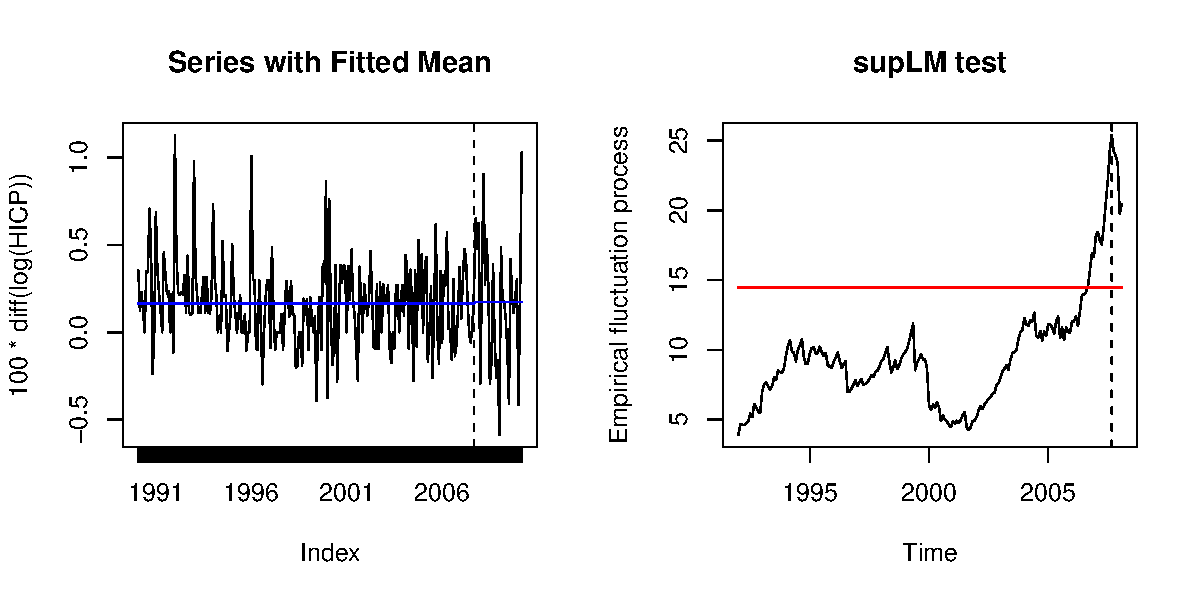
\includegraphics{results-012.pdf}
  \caption{Series and supLM test for Austria}
  \label{aut}
\end{figure}

The reason for this is a strong increase in the yearly Austrian inflation rate following a heavy increase in oil price which was further amplified by a rise of mineral taxes. However, we fail to find any evidence for an incrase in mean or volatility of the Austrian rate following the introduction of the Euro paper money. \\
Lets consider Slovenia as the first Eastern European country that introduced the Euro. In August 2003 the new regime started with a much lower mean value (only a third now of its previous value) and interestingly enough, a higher volatility. 

\begin{figure}[ht!p]
  \centering
    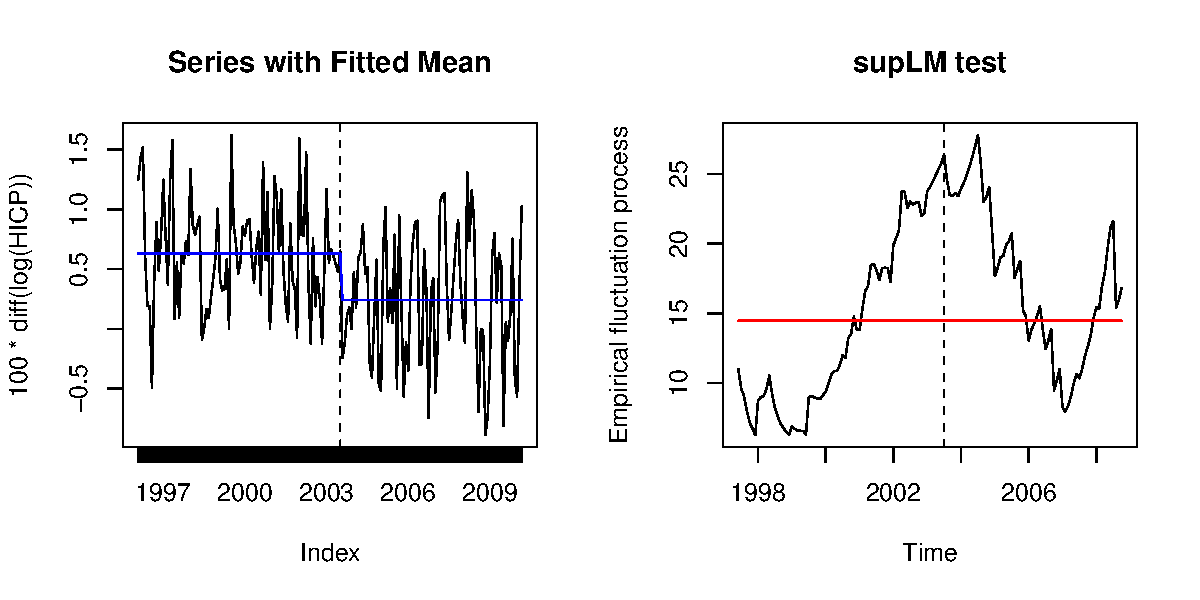
\includegraphics{results-131.pdf}
  \caption{Series and supLM test for Slovenia}
  \label{aut}
\end{figure}

%
%The LWZ criteria favors one break. 
%
%
%\begin{figure}[ht!p]
%  \centering
%    \includegraphics{results-132.pdf}
%  \caption{LWZ and Negative Log-Likelihood for Break Point Selection}
%  \label{aut}
%\end{figure}

Slovenia is a good example of the benefits of an early Euro adoption. Its efforts to meet the criterias as set forth in the Maastricht treaty were successfull, actually Slovenia reached them in 2005. So from 2003 onwards inflation was lower but with a much higher variance. Regarding the dating in 2003, we have to keep in mind that this was the year where most of the financial reforms were introduced. Slovenia seems to be the only case where the introduction of the Euro was followed by an increase in yearly inflation, which faded away following the financial crises and its deflationary effects. \\


%As a last example we focus on Spain. \\


%Other possible explanations: 
%
%- rise in value added tax (VAT; as in Germany in 2007)
%- change in central bank policy (for example Spain changed to inflation targeting in 1995; Uk, Swe and Finland in 1992)
%- role of budget deficits

% Quelle f�r diese Behaupunten: http://www.oenb.at/isaweb/dyna2.do?go=initIndikatoren&definitionLaden=false&hierarchieIdSelected=108

Another possible explanation pattern could be the growth in the  money supply. A drawback is the current lack of data\footnote{hopefully to be solved}. But for some countries we can find some plausible findings. Regarding the case of Denmark, the M1 money supply started contracting in June 2000 (on a monthly base). In Estonia we find the highpoint in M3 expansion ending with March 1998, with much lower M3 growth rates afterwards. The same happended to Hungary in April and May 1998. In the Polnish case we find a severe contraction of the money supply in May 2001. Similar findings hold true for Germany as well. \\
In Spain we see a stronger increase in M1 in May and June 1996 (nothing for the other break, data scarceity). In Portugal we find a modest increase in year on year M1 money supply growth starting in July 1992. We find nothing peculiar for Slovakia and Hungary. In Estonia the M1 money supply starts to contract severely on a yearly base following March 1998. In Slovenia we find a contraction of the Money Supply in July 2003, with the whole year 2003 witnessing a sharp decrease in the year on year growth. Poland starts contracting the year on year M1 money supply after June 2000 with very low growth rates till January 2002. 

%\readme{irgendwo noch inne (nach \cite{duarte}), dass es normal isch, dass die relativen Preise fluktuieren, got uf asymmetrische productivity shocks zruck}


% for denmark: see: C:\Dissertation\Daten\DSI\M1\daten - the denmark analysis, alos: Spain, Portugal, Slovakia, Hungary Estonia noch am absatz f�r M1

Concerning monetary unions, it is interesting to notice that Belgium and Luxembourg, that constituted a monetary union prior to the European Monetary Union, did not experience the same timing in their break towards a higher mean and a significantly higher volatility regime. 

With regard to the alleged benefit of monetary unions, the import of credibility to former high inflation countries (like Italy and Spain), did nothing to decrease their mean or volatility, rather to the contrary. Spain and Italy did have a -- rather -- low mean low volatility regime from 1996:6 to 2000:12 but then things changed towards higher volatility. It appears as if both countries tried to decrease inflation prior to the fixing of the exchange rates and let go afterwards.  

Following the reasoning of a study by \cite{duarte}, high volatility of inflation rates within regions of a union may be explained a countries decision to lower the inflation differential by means of fiscal policy. This explanation might fit to Spain and Italy, both were above the the average EU inflation. 


% Quelle: f�r Deutschland M3 bis 1995
%http://www.bundesbank.de/statistik/statistik_zeitreihen.php?lang=de&open=ewu&func=row&tr=TSD304
%
%Deutschland: M3 bis 1995
%dort ersichtlihc, dass Deutschland zu Bruchzeitpunkten jeweils �nderungen im m3 aggregat hat


%The AR distances table, measuring the similarity of short--run inflation dynamics as in \citet{palomba} more or less supports this group building, although it is much more accurate. The similarity of the structural breaks thus is interesting topic for future research. 

%give the 3 most similar in AR distances: in Palomba Paper (table 2)
%
%Italy: Greece, France, Portugal
%Poland: Ireland, Spain, UK
%Sweden: Denmark, Netherlands, UK
%Netherlands: Sweden, UK, Portugal
%France: Italy, Greece, Belgium
%
%
%either support or not support group 1
%AR distance: the lower the more similar
%

\clearpage
\section{Conlcusion}


\clearpage
\bibliography{papers}

\clearpage


\end{document}
